\documentclass[../main.tex]{subfiles}
\begin{document}
\chapter{Soluzione proposta}

In questo capitolo viene presentato il programma di conversione. La prima parte descrive le scelte effettuate per convertire i campi nell'altro formato e come automatizzare la procedura. La seconda parte introduce il concetto di programmazione parallela e le possibili soluzioni per rendere efficiente la conversione.


\section{Conversione}
Per convertire i file di nProbe nel formato utilizzato da Argus si è fatto per prima cosa uno studio sui campi degli header per individuarne le differenze. Alcuni campi sono presenti in entrambi i formati seppure con nome diverso, altri sono stati ottenuti come combinazione, mentre quelli che nProbe utilizza in più rispetto ad Argus sono stati scartati. 

Il primo campo di Argus è il campo \textit{StartTime}. Il corrispondente campo usato da nProbe è \textit{FIRST\_SWITCHED}. In figura ~\ref{fig:starttime} vengono descritte le formattazione dei 2 campi.
\begin{figure}[H]
				\centering
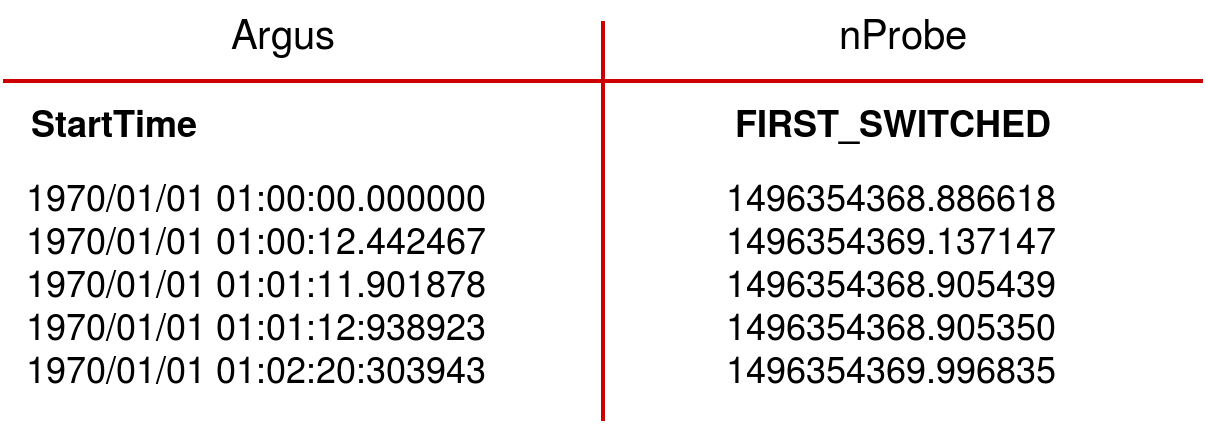
\includegraphics[scale=0.32]{starttime.png}
				\caption{Formattazione delle date}
				\label{fig:starttime}
\end{figure}
Argus salva la data seguita da uno spazio bianco, le ore i minuti e i secondi e i microsecondi. nProbe invece non salva la data ma soltanto i secondi nel formato $10^{10}$ con i microsecondi. Per effettuare una conversione precisa dei 2 campi la data nel formato YYYY/MM/DD è stata presa dalla struttura gerarchica delle cartelle guardando in modo ricorsivo la posizione del file all'interno del file system. Per i secondi si è convertito i 10 gigasecondi in secondi, mentre per i microsecondi non c'è stato bisogno di conversione.

Il secondo campo di Argus è \textit{Duration}. Non esistendo un campo di nProbe che indica la durata si è usata la differenza tra i campi \textit{LAST\_SWITCHED} e \textit{FIRST\_SWITCHED}. In figura ~\ref{fig:duration} viene mostrata l'operazione di differenza.
\begin{figure}[H]
				\centering
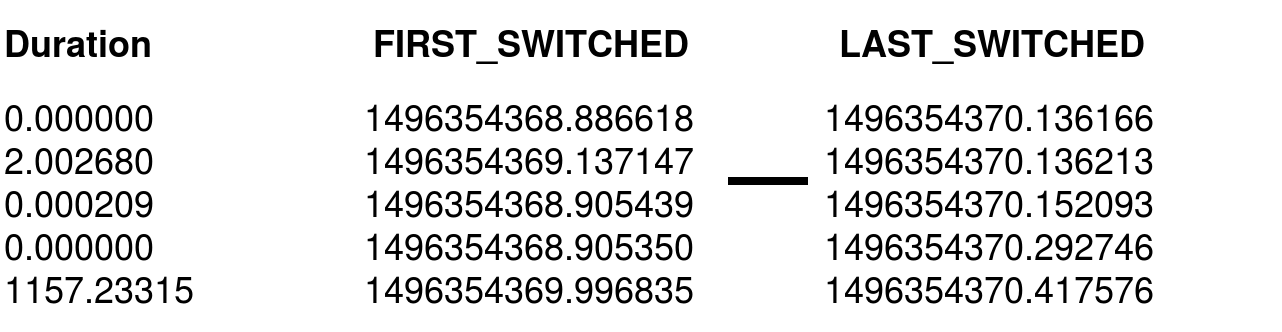
\includegraphics[scale=0.33]{duration.png}
				\caption{Durata}
				\label{fig:duration}
\end{figure}
Dopo aver fatto la differenza tra i 2 campi si converte il risultato in secondi e microsecondi per rispettare il formato di Argus.

Il terzo campo di Argus è \textit{Proto} che indica il protocollo usato dalla connessione. Argus salva in questo campo la keyword del protocollo mentre nProbe salva il numero decimale. La figura ~\ref{fig:protocol} mostra la differenza tra i 2 formati.
\begin{figure}[H]
				\centering
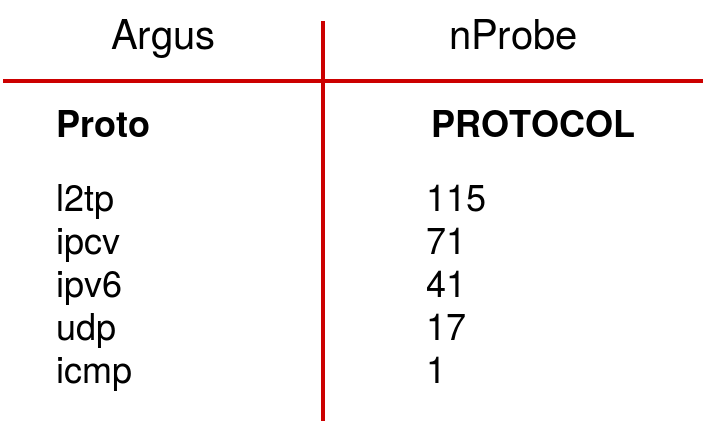
\includegraphics[scale=0.33]{protocol.png}
				\caption{Protocolli}
				\label{fig:protocol}
\end{figure}
Per effettuare la conversione tra numeri e keyword si è usato un \textit{dictionary}, un costrutto del linguaggio Python. Questa particolare struttura dati è un array associativo in cui una chiave viene associata ad un valore. Come chiave si è usato il numero decimale del protocollo e come valore la keyword. Il costo medio di accesso ad un valore con questa struttura dati è $\mathcal{O}(1)$. La figura ~\ref{lst:dictionary} rappresenta la sintassi di un dictionary in Python.
\lstinputlisting[language=Python, firstline=32, lastline=43, label={lst:dictionary}, caption={Esempio di dictionary}]{singlecore.py}

Il quarto campo di Argus è \textit{SrcAddr} che indica l'indirizzo IP sorgente. Questo campo è presente nei campi di nProbe, di conseguenza non è necessario effettuare una conversione. 

Il quinto campo di Argus è \textit{Sport} che indica la porta di origine della connessione. Il campo corrispettivo di nProbe è \textit{L4\_SRC\_PORT} e condividono entrambi lo stesso formato, non è pertanto necessario alcun tipo di conversione per questi 2 campi.

Il sesto campo di Argus si chiama \textit{Dir} e rappresenta la direzione della connessione. Per la conversione si è utilizzato il campo di nProbe \textit{BIFLOW\_DIRECTION}. In nProbe si ha come valore del campo BIFLOW\_DIRECTION solo 1 e 2. Il numero 1 indica un flow monodirezionale che va dall'indirizzo sorgente al indirizzo destinazione, mentre il valore 2 indica un flow bidirezionale. In Argus si hanno più valori:
\begin{itemize}
				\item \textbf{-} la connessione è normale
				\item $\boldsymbol|$ la connessione è stata resettata
				\item \textbf{o} la connessione è scaduta
				\item \textbf{?} la direzione della connessione è sconosciuta
\end{itemize}

La figura ~\ref{fig:direction} mostra come è stata effettuata la conversione.
\begin{figure}[H]
				\centering
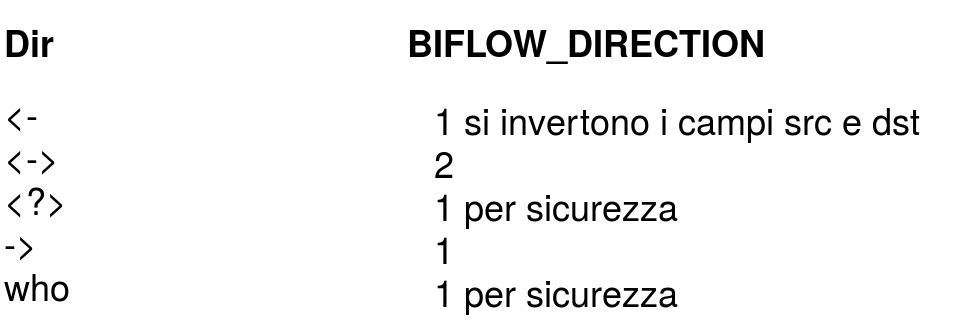
\includegraphics[scale=0.36]{direction.png}
				\caption{Direzione connessione}
				\label{fig:direction}
\end{figure}
Nel primo caso si può convertire con 1 ma bisogna invertire i campi src e dst perchè la connessione viene inizializzata a sinistra. Nel secondo caso si converte con 2 perchè il flow è bidirezionale. Nel terzo caso la direzione della connessione è sconosciuta, si è scelto di convertire con 1 per sicurezza e non lasciare il campo vuoto. Nel quarto caso il flow è monodirezionale e quindi si converte con 1. Nell'ultimo caso \textit{who} è una keyword che indica una comunicazione \textit{icmp} che non viene utilizzata da Stratosphere, si è scelto di convertire con 1 per sicurezza.

Il settimo campo di Argus è \textit{DstAddr} e rappresenta l'indirizzo IP di destinazione. Il campo corrispondente di nProbe si chiama \textit{IPV4\_DST\_ADDR}. Come nel caso dell'indirizzo IP sorgente anche qui non è necessaria la conversione.

L'ottavo campo di Argus è \textit{Dport} e indica la porta di destinazione. Argus usa una formattazione decimale, stessa cosa il campo \textit{DST\_PORT} di nProbe.

Il nono campo di Argus è \textit{State} e denota lo stato della connessione. Questo campo non è generabile a partire dai file di nProbe. Per effettuare questa conversione si è prima verificato l'impatto di questo campo nella generazione dei modelli di STF inserendo un valore non corretto. I modelli generati cambiando i valori di questo campo con valori non corretti restano invariati, pertanto il campo State non ne influenza la generazione. Per la conversione si è quindi inserito un valore costante "CON" per sicurezza. La figura ~\ref{fig:state} mostra esempi di valori del campo State di Argus.
\begin{figure}[H]
				\centering
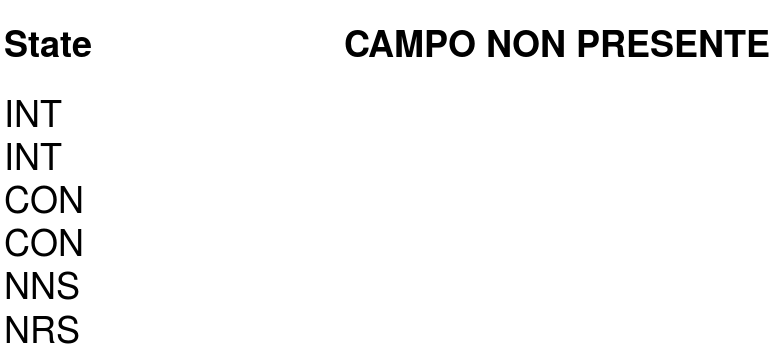
\includegraphics[scale=0.36]{state.png}
				\caption{Stato connessione}
				\label{fig:state}
\end{figure}

Il decimo e undicesimo campo di Argus sono \textit{sTos} \textit{dTos} e rappresentano il \textit{Type of Service} sorgente e destinazione di un pacchetto. Questi campi sono presenti in nProbe e condividono la stessa formattazione di Argus, non è pertanto necessaria una conversione.

Il dodicesimo campo di Argus è \textit{TotPkts} e rappresenta i pacchetti totali transitati nella connessione. Questo campo non compare in nProbe che ha però i campi \textit{IN\_PKTS} e \textit{OUT\_PKTS}. Per fare la conversione da nProbe ad Argus si sono sommati questi 2 valori per ottenere il totale dei pacchetti. La figura ~\ref{fig:totpkts} mostra l'operazione di somma e la formattazione dei dati.
\begin{figure}[H]
				\centering
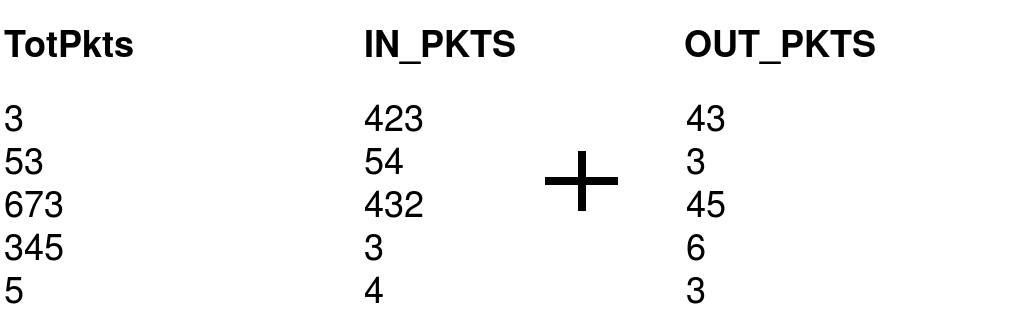
\includegraphics[scale=0.36]{totpkts.png}
				\caption{Pacchetti totali transitati nella connessione}
				\label{fig:totpkts}
\end{figure}

Il tredicesimo campo di Argus è \textit{TotBytes} e rappresenta i bytes totali transitati nella connessione. Come visto per il campo TotPkts, in nProbe questo campo non campare direttamente ma sono presenti \textit{IN\_BYTES} e \textit{OUT\_BYTES}. Per fare la conversione questi 2 campi vengono sommati per ottenere il totale. La figura ~\ref{fig:totbytes} mostra l'operazione di somma e la formattazione dei dati.
\begin{figure}[H]
				\centering
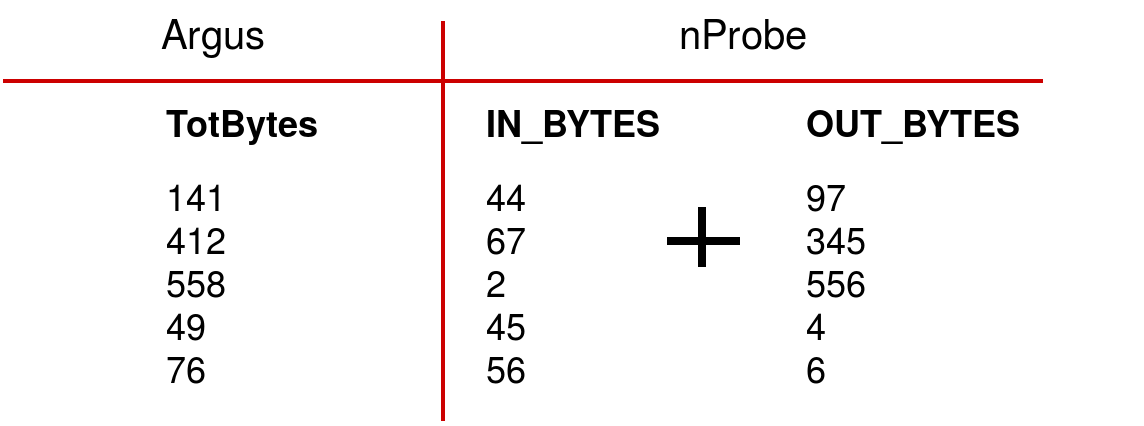
\includegraphics[scale=0.36]{totbytes.png}
				\caption{Bytes totali transitati nella connessione}
				\label{fig:totbytes}
\end{figure}

Il quattordicesimo campo di Argus è \textit{SrcBytes} che indica i bytes in entrata dal sorgente. Per fare questa conversione si è usato il campo di nProbe \textit{IN\_BYTES} in figura ~\ref{fig:totbytes}.

Il quindicesimo e ultimo campo di Argus è il campo label che serve per i metadata. Questo campo non è presente in nProbe e non è necessario per la generazione dei modelli, viene quindi lasciato vuoto.



\section{Automatizzazione conversione}
La conversione è stata automatizzata con la scrittura di uno script in Python. Si è scelto di scrivere un programma usando questo linguaggio per la facilità di utilizzo nel lavorare con i file e per le performance.

\subsection{Lettura dei file}\label{letturafilesec}
Il problema richiede lo sviluppo di un programma che converte file in modalità batch.
La figura ~\ref{fig:lettura} rappresenta l'operazione da eseguire per la lettura dei file. I file, che sono organizzati in cartelle per data, sono presi in modo ricorsivo e inseriti in una coda. Al termine della lettura dei file si ha una coda con l'insieme dei path dei file da leggere.
\begin{figure}[H]
				\centering
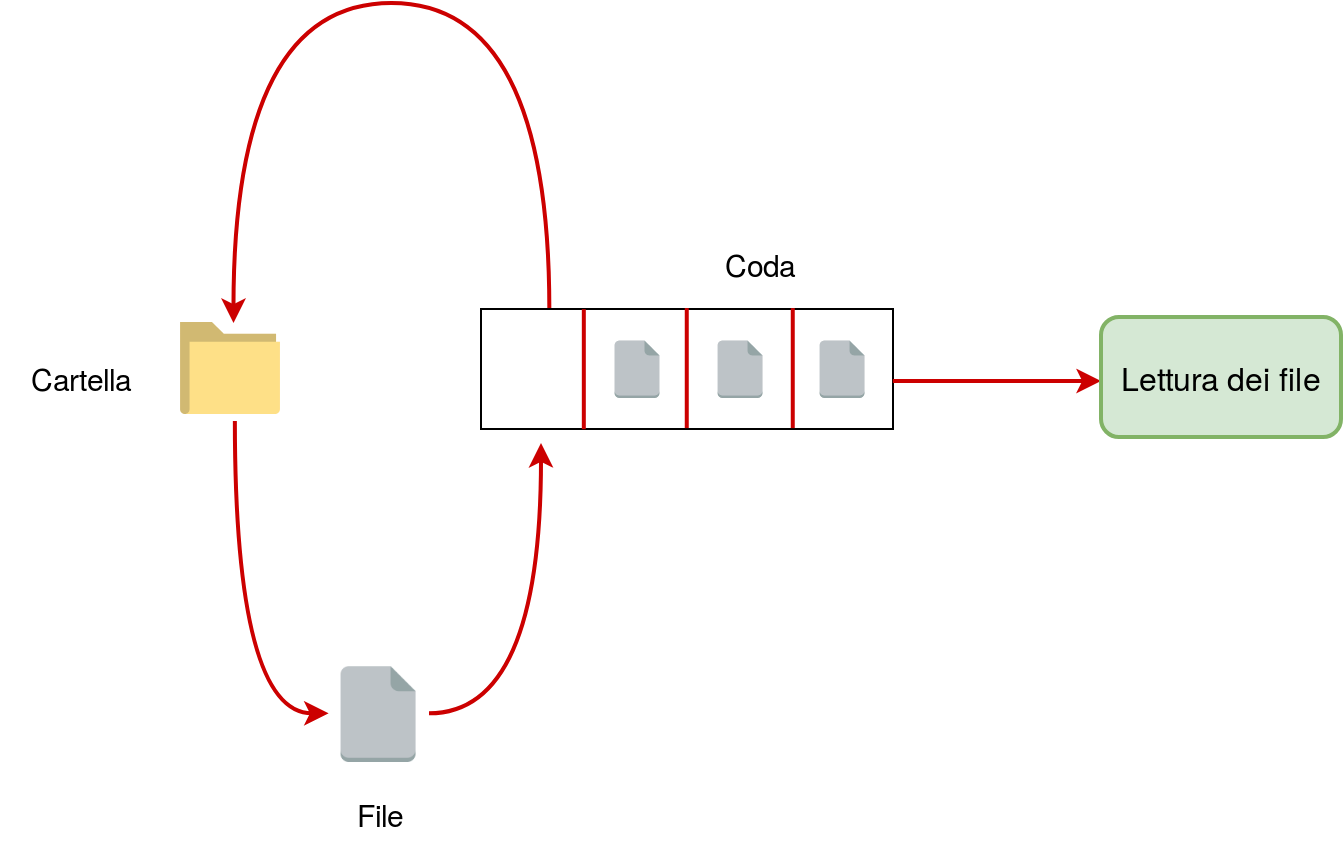
\includegraphics[scale=0.3]{lettura.png}
				\caption{Lettura dei file ricorsiva}
				\label{fig:lettura}
\end{figure}

Lo pseudocodice ~\ref{alg:ricorsione} descrive l'immagine ~\ref{fig:lettura}. Alla riga 1 si assegna ad una variabile il path della cartella in cui sono contenuti i file e nella seconda riga si crea un oggetto coda \cite{queuedef}. Si creano poi 2 cicli \textit{for} annidati che scorrono la struttura gerarchica della cartella e per ogni ogni file all'interno della cartella \textit{minuti} si mette in coda il file. Quando l'esecuzione dei 2 cicli \textit{for} finisce rimane una coda con all'interno tutti i path dei file.
\begin{algorithm}
\caption{Inserimento file in una coda}
				\label{alg:ricorsione}
				\hspace*{\algorithmicindent} \textbf{Input}: la variabile pathCartella è il percorso della cartella che fornisce l'utente \\
\begin{algorithmic}[1]
				\State $\textit{cartellaRoot} \gets $\textit{pathCartella}
				\State $\textit{Coda} \gets $\textit{Queue()} \Comment{inizializza una coda}
				\For{\texttt{mesi, giorni, minuti in \textit{cartellaRoot}}}
						\For{\texttt{file in minuti}}
						\State $\textit{Coda}.append() \gets $\textit{file} \Comment{inserisce il file nella coda}
						\EndFor
				\EndFor
\end{algorithmic}
\end{algorithm}

\subsection{Lettura righe dei file} 
Una volta che la coda è completa si passa alla lettura dei file. Per questa operazione si prende un file file dalla coda e si legge una riga alla volta. Da ogni riga vengono estratti i campi utili alla conversione.
La figura ~\ref{fig:letturarighe} descrive questa operazione. Si è scelto di leggere i file per righe e non per intero perchè sono troppo grandi e rischiano di saturare la RAM, soprattutto leggendo più file in contemporanea. La soluzione scelta permette di eseguire l'algoritmo anche su computer con poca RAM.

\begin{figure}[H]
				\centering
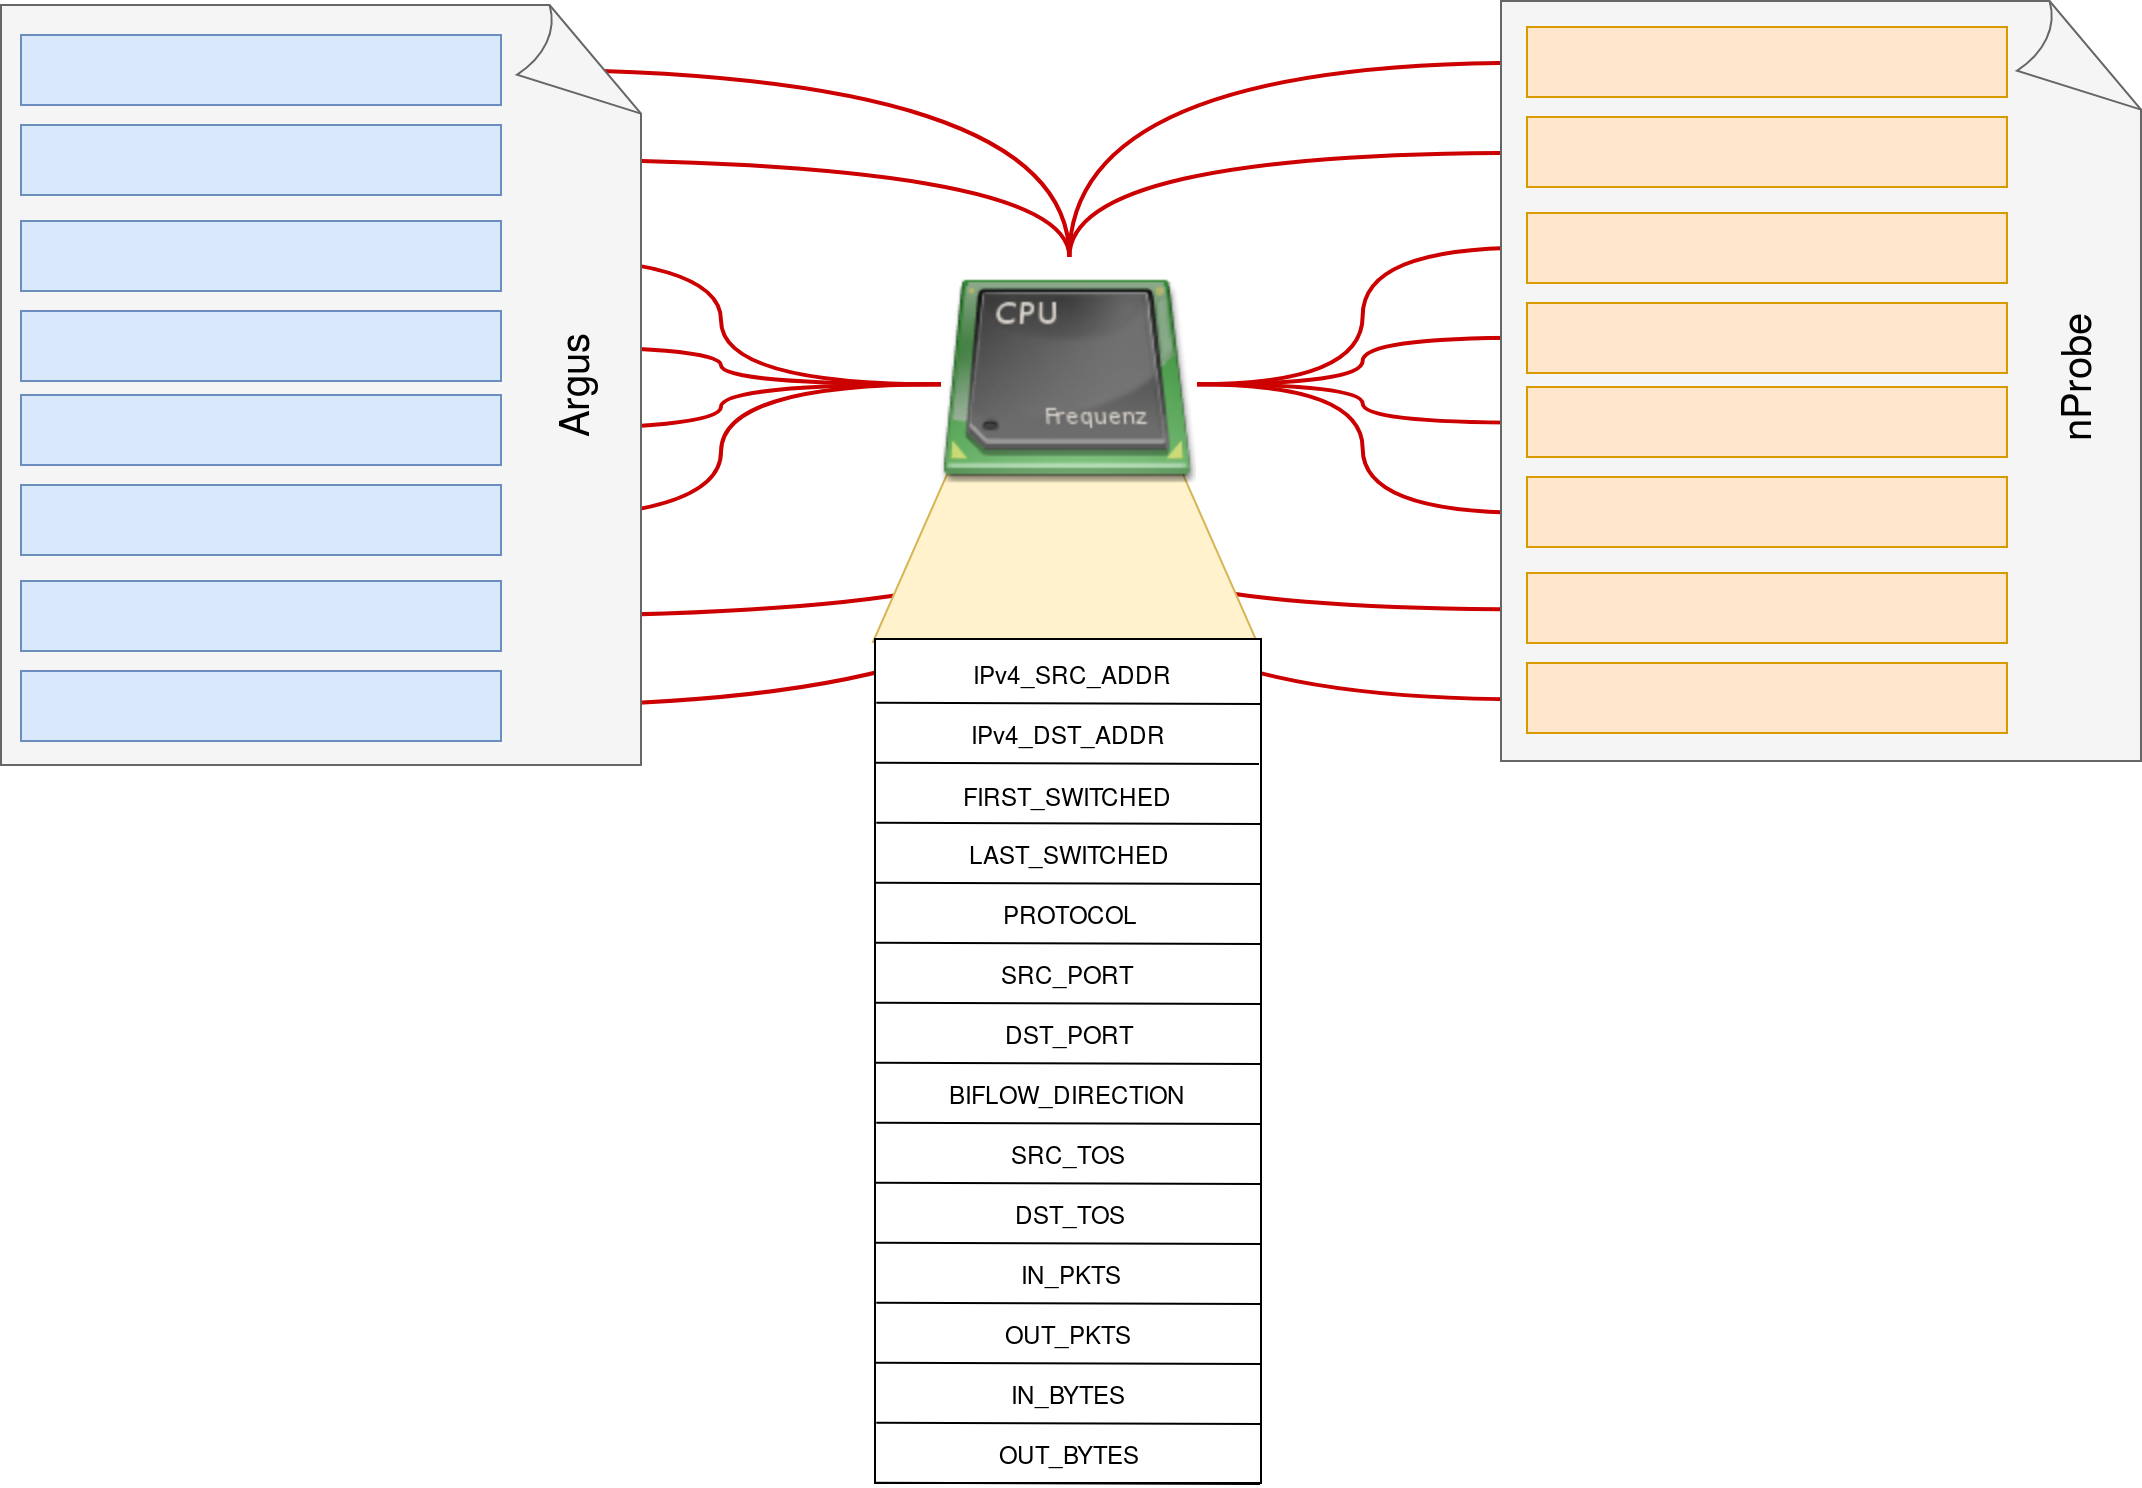
\includegraphics[scale=0.27]{letturarighe.png}
				\caption{Lettura delle righe}
				\label{fig:letturarighe}
\end{figure}


Lo pseudocodice ~\ref{alg:pseudocodicelettura} descrive l'immagine ~\ref{fig:letturarighe}. Si inizializza una lista per ogni campo di nProbe da leggere e si prende un file dalla coda. Per ogni riga del file si aggiunge il campo letto alla lista. Finito il ciclo for le liste contengono tutti i campi del file.

\begin{algorithm}[H]
\caption{Lettura righe file}
				\label{alg:pseudocodicelettura}
\begin{algorithmic}[1]
				\State inizializzazione di una lista per ogni campo
				\State $\textit{file} \gets $Coda.get() \Comment{prende un file dalla coda}

				\For{\texttt{riga in \textit{file}}}
						\State Assegna ad ogni lista il valore letto dalla riga
				\EndFor
\end{algorithmic}
\end{algorithm}

\subsection{Conversione dei dati}
Lo pseudocodice ~\ref{alg:pseudocodiceconversione} descrive il processo di conversione che si effettua sui valori letti nel codice ~\ref{alg:pseudocodicelettura}. La data si ricava dal nome delle cartelle scomponendo il path, la figura ~\ref{fig:conversioneschema} mostra l'acquisizione della data partendo dal percorso del file. Per ogni riga viene poi fatta una addizione dei pacchetti e dei byte in entrata e in uscita.
\begin{figure}[H]
				\centering
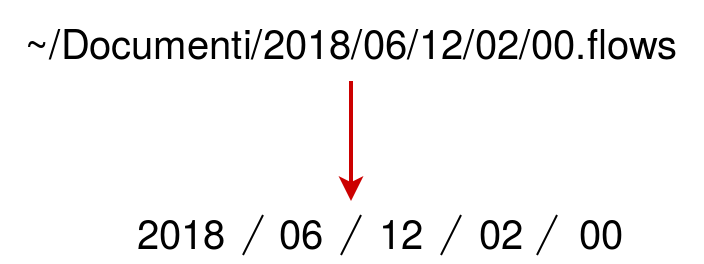
\includegraphics[scale=0.27]{conversioneschema.png}
				\caption{Acquisizione data dal percorso del file}
				\label{fig:conversioneschema}
\end{figure}

\begin{algorithm}[H]
				\caption{Conversione dei campi}
				\label{alg:pseudocodiceconversione}
\begin{algorithmic}[1]
				\State scomposizione del percorso file per ricavare la data
				\While {i $<$ lunghezza del file}
				\State $\textit{last} \gets $\textit{last\_switched[i]} \Comment{assegna il valore i-esimo alla variabile}
				\State $\textit{first} \gets $first\_switched[i]
				\State $\textit{tot\_pkts} \gets $in\_pkts[i] + out\_pkts[i]
				\State $\textit{tot\_bytes} \gets $in\_bytes[i] + out\_bytes[i]
				\EndWhile
\end{algorithmic}
\end{algorithm}

\subsection{Scrittura su file}
La figura ~\ref{fig:conversionetonprobe} mostra il procedimento di scrittura su file. Questo passaggio viene effettuato finita la conversione dei file.
\begin{figure}[H]
				\centering
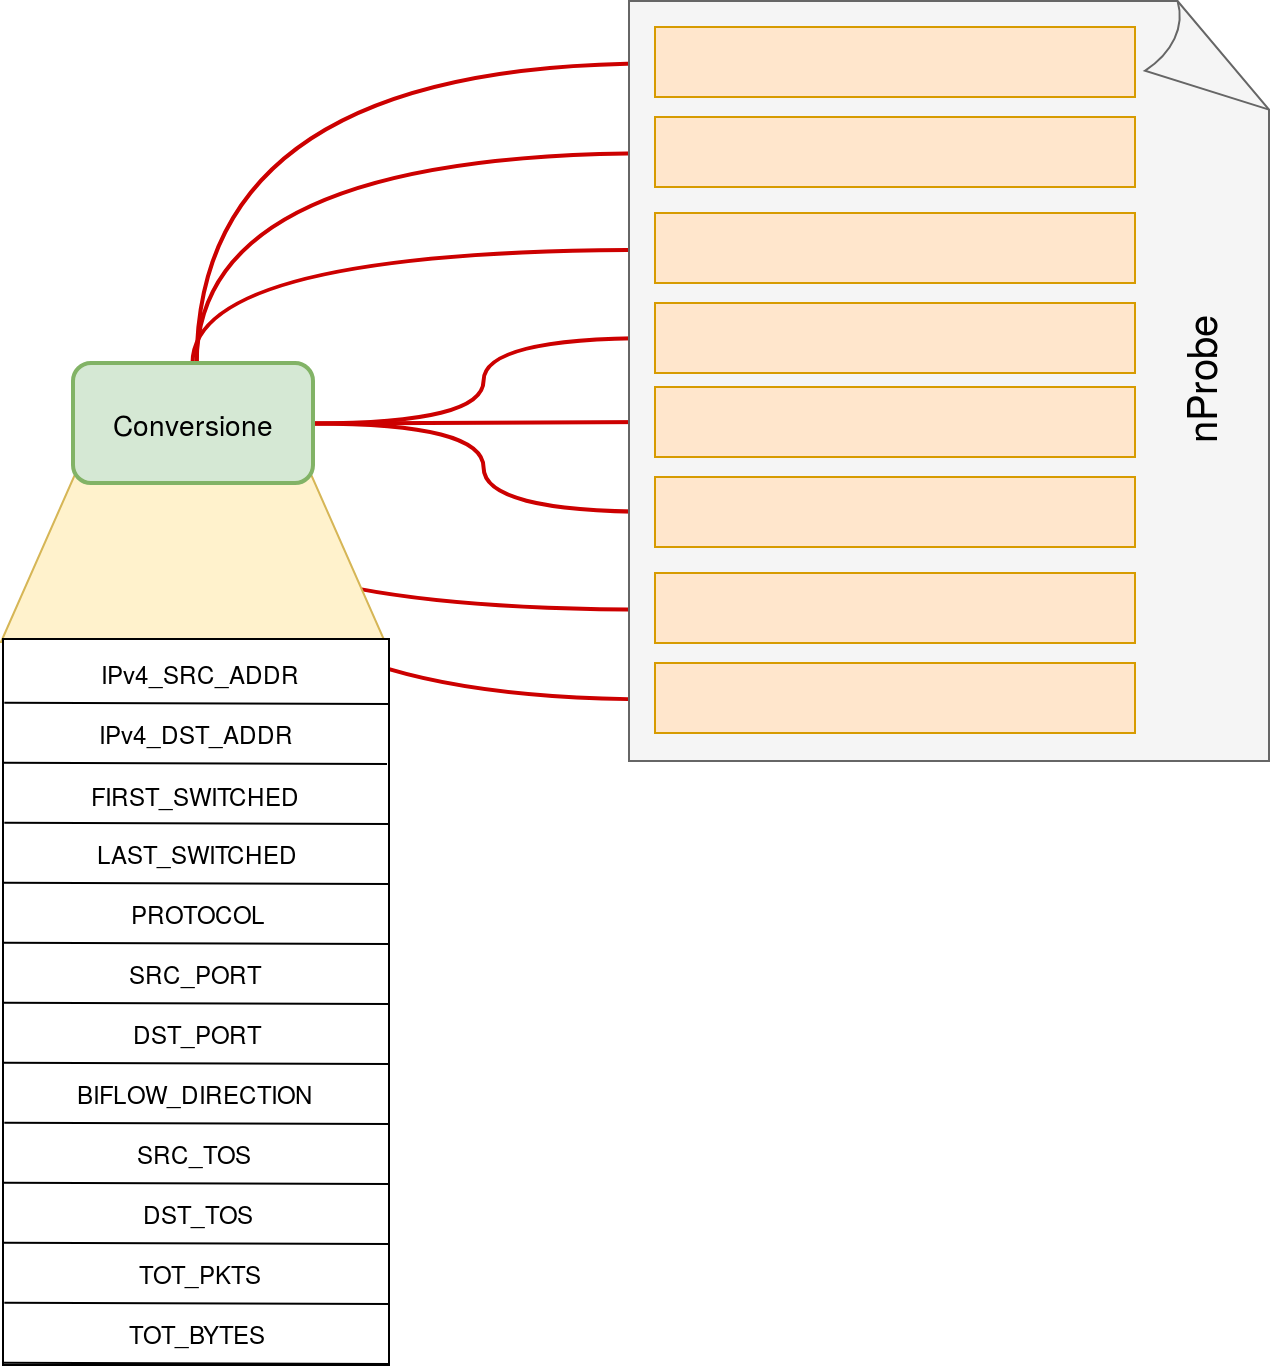
\includegraphics[scale=0.27]{conversionetonprobe.png}
				\caption{Scrittura su file nProbe}
				\label{fig:conversionetonprobe}
\end{figure}

Lo pseudocodice ~\ref{alg:pseudocodicescrittura} descrive il processo di scrittura su file. All'interno di un ciclo \textit{while} si effettua una scrittura di tutti i campi convertiti nel passaggio precedente.
\begin{algorithm}[H]
				\caption{Scrittura su file}
				\label{alg:pseudocodicescrittura}
\begin{algorithmic}[1]
				\While {$i < lunghezza del file$}
				\State scrive la conversione su file
				\EndWhile
\end{algorithmic}
\end{algorithm}

\subsection{Algoritmo completo}
La figura ~\ref{fig:soluzioneproposta} mostra lo schema completo per la risoluzione dell'algoritmo.
\begin{figure}[H]
				\centering
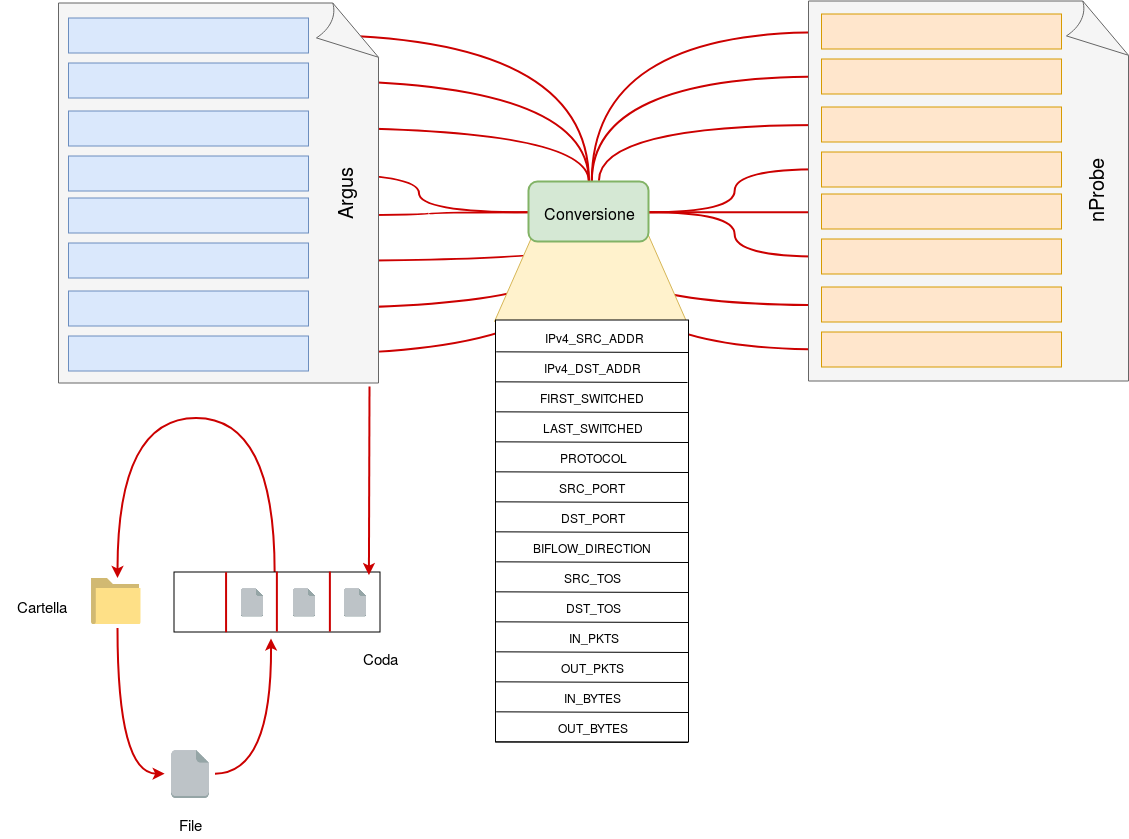
\includegraphics[scale=0.35]{soluzioneproposta.png}
				\caption{Schema completo}
				\label{fig:soluzioneproposta}
\end{figure}

L'algoritmo ~\ref{alg:pseudocodicecompleto} scritto in pseudocodice descrive una soluzione single core al problema

\begin{algorithm}[H]
\begin{algorithmic}[1]
				\caption{Pseudocodice completo}
				\label{alg:pseudocodicecompleto}
				\State $\textit{cartellaRoot} \gets $\textit{pathCartella}
				\State $\textit{Coda} \gets $\textit{Queue()} \Comment{inizializza una coda}
				\For{\texttt{mesi, giorni, minuti in \textit{cartellaRoot}}}
						\For{\texttt{file in minuti}}
						\State $\textit{Coda}.append() \gets $\textit{file} \Comment{inserisce il file nella coda}
						\EndFor
				\EndFor
				\State inizializzazione di una lista per ogni campo
				\State $\textit{file} \gets $Coda.get() \Comment{prende un file dalla coda}

				\For{\texttt{riga in \textit{file}}}
						\State Assegna ad ogni lista il valore letto dalla riga
				\EndFor
				\State scomposizione del percorso file per ricavare la data
				\While {i $<$ lunghezza del file}
				\State $\textit{last} \gets $\textit{last\_switched[i]} \Comment{assegna il valore i-esimo alla variabile}
				\State $\textit{first} \gets $first\_switched[i]
				\State $\textit{tot\_pkts} \gets $in\_pkts[i] + out\_pkts[i]
				\State $\textit{tot\_bytes} \gets $in\_bytes[i] + out\_bytes[i]
				\EndWhile
				\While {$i < lunghezza del file$}
				\State scrive la conversione su file
				\EndWhile
				
\end{algorithmic}
\end{algorithm}

\section{Rendere efficiente la conversione}

Nel programma descritto in precendenza viene generato un solo file di output in cui vengono convertiti tutti i file dati in input. Questa soluzione è comoda perchè da migliaia di file si ottiene un solo file con i dati convertiti, ma presenta il problema di creare un file con dimensioni enormi e di difficile gestione (il file può raggiungere dimensioni tali da rendere difficile anche solo aprirlo in lettura).


Il programma è inoltre inefficiente poichè è single core e ha come collo di bottiglia la scrittura su un unico file. 
La soluzione proposta seppure sia teoricamente corretta non può avere un'applicazione nel mondo reale. Bisogna cambiare quindi strategia per rendere la conversione più veloce sfruttando le macchine multi core e per avere in output file di dimensioni accettabili.

\subsection{Possibili soluzioni}
Si possono pensare diverse soluzioni che migliorerebbero in modo significativo il programma visto in precedenza:

\begin{itemize}
				\item Lavorare su chunk di file
				\item Meccanismi di lock
				\item Scrittura su file 1:1
\end{itemize}

\begin{verse}
\textbf{Lavorare su chunk di file}
Per velocizzare il programma e sfruttare i processori disponibili si potrebbe assegnare ad ogni processore un file da leggere e convertire. Quando il processore termina la conversione dei dati scrive sul file in output. In questo modo si dividrebbe il tempo di esecuzione sul numero di processori disponibili. 
Questa soluzione rende il più veloce possibile la conversione dei file ma i processori finiscono per scrivere sullo stesso file senza avere nessuna regola di precedenza, questo crea problemi perchè le scritture in output non sono ordinate e non è possibile creare modelli comportamentali affidabili. Le scritture su file devono essere ordinate e sequenziali, inoltre questa soluzione ha il problema di scrivere sempre su unico file e, come detto in precedenza, questo tipo di soluzione non è possibile.
\end{verse}

\begin{verse}
\textbf{Meccanismi di lock}
Un modo per risolvere i problemi precedenti è quello di utilizzare il concetto di semaforo. 
In informatica un semaforo è un tipo di dato astratto gestito da un sistema operativo multitasking per sincronizzare l'accesso a risorse condivise tra processi. È composto da una variabile intera e da una coda di processi. Quando un processo apre il file per scriverci viene impostato un semaforo che segnala che la risorsa è occupata, se un altro processore prova ad aprire lo stesso file per scriverci gli sarà negato l'accesso dal semaforo fino a quando l'altro processo non rilascerà la risorsa.
In questo modo si risolve il problema delle scritture ordinate, ma c'è da tener conto che i semafori riducono la velocità di esecuzione dell'algoritmo poichè mentre un processore occupa la risorsa tutti gli altri processori devono mettersi in coda per aspettarne il rilascio. Nonostante questa soluzione rallenti l'esecuzione del programma rispetto alla soluzione precedente è comunque molto più veloce della versione single core perchè, sebbene la scrittura su file sia rallentata dai semafori, si guadagna molto tempo nella lettura e conversione dei dati dove non ne è necessario l'utilizzo, e che quindi viene effettuata alla massima velocità possibile. Questa soluzione risolve anche il problema dell'ordinamento delle scritture.
Rimane il problema della scrittura su un unico file che però può essere risolto facilmente decidendo di scrivere su un nuovo file quando raggiunge una dimensione specificata.
Se si implementa la divisione del file di output questa soluzione può considerarsi efficiente anche se rimane il collo di bottiglia introdotto dai semafori che costringe i processi ad aspettare in coda quando una risorsa è impegnata.
\end{verse}

\begin{verse}
\textbf{Scrittura su file 1:1}
In questa soluzione ogni processore apre un file, lo legge, lo converte e scrive su un proprio file.
Questa soluzione è decisamente la più semplice tra quelle proposte ed è anche la più efficiente poichè i processori non entrano mai in conflitto tra di loro cosicchè da effettuare letture, conversioni e scritture alla massima velocità possibile dalla macchina.
Un problema che può creare questa soluzione è la produzione di una grande quantità di file in output. Si pensi che una sola settimana di traffico di rete, sono circa 10 mila file.
\end{verse}

\subsection{Scelta effettuata}

Si è scelto di procedere con l'ultima soluzione presentata perchè data la grande quantità di informazioni da convertire si preferisce l'approccio più veloce a discapito dell'ordinamento finale.

Per realizzare questa soluzione si effettua una lettura analoga dei file vista nella sezione ~\ref{letturafilesec} per creare una coda che contiene il percorso di tutti i file presenti in un cartella. Si chiama poi una funzione che prende un numero designato di core da assegnare ad una funzione. Ogni core prende un file all'interno della coda, lo legge, lo converte e scrive su un file in modo indipendente dagli altri.
La figura ~\ref{fig:multiCore} mostra la parallelizzazione dell'algoritmo.

\begin{figure}[H]
				\centering
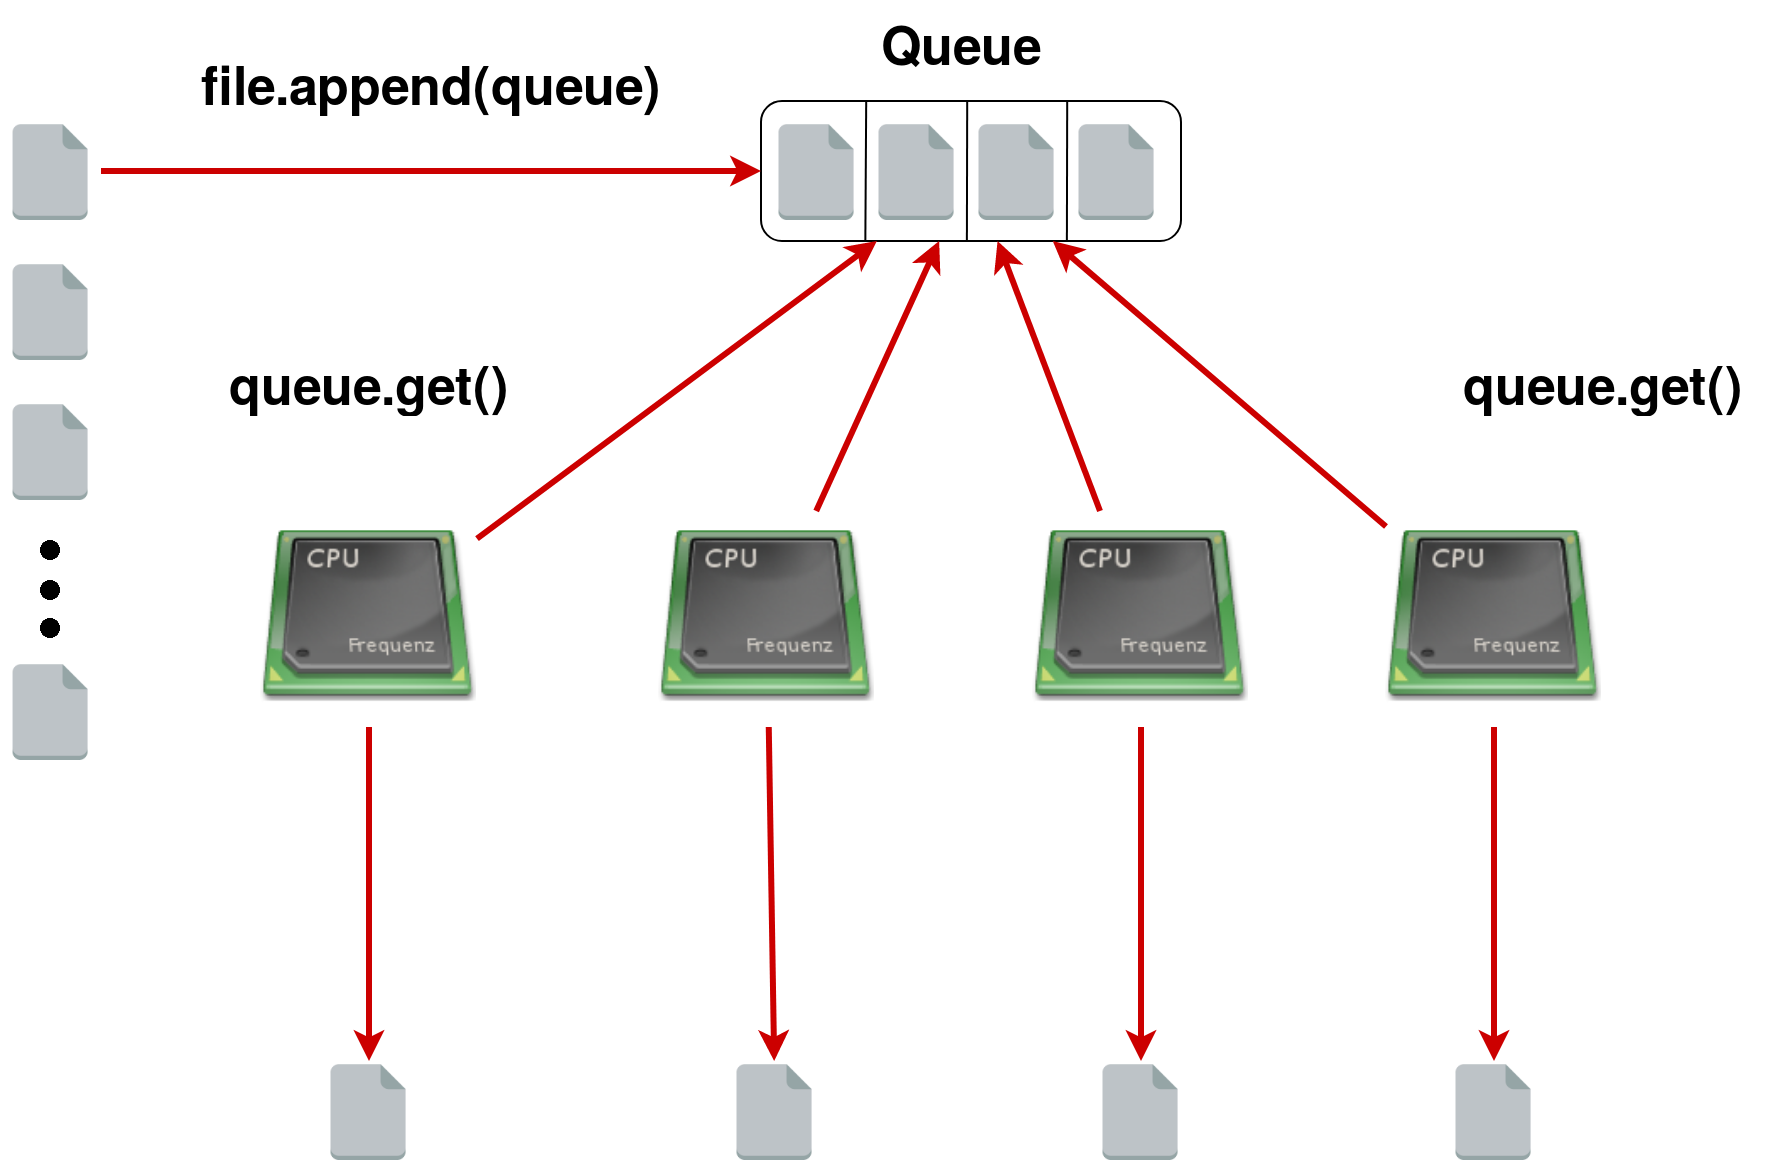
\includegraphics[scale=0.22]{hydra.png}
				\caption{Multi core version}
				\label{fig:multiCore}
\end{figure}

Lo pseudocodice ~\ref{alg:multiCore} descrive questa soluzione.
\begin{algorithm}[H]
\caption{Multi core version}
				\label{alg:multiCore}
\begin{algorithmic}[1]
\Procedure{Hydra}{}
\ForAll{\textit{file} in path}
\State $\textit{Queue[]} \gets \textit{file}$
\State legge i dati dal $\textit{file}$
\State prende $n$-core
\While{\textit{Queue[]} $\textbf{not empty}$}
\State $\textit{filename} \gets $\textit{Queue.get()}
\State converte i dati nel nuovo formato
\State scrive i dati in un nuovo file
\EndWhile
\EndFor
\EndProcedure
\end{algorithmic}
\end{algorithm}

\section{Correzione del codice sorgente}

Il codice sorgente è stato modificato per poter effettuare una installazione funzionante.
Per la scrittura di questa tesi si è scaricata la versione più aggiornata disponibile sulla pagina GitHub di slips \cite{slipscurrent}. Questa versione, essendo in alpha, non funziona \textit{out of the box}. È stato perciò necessario apportare delle modifiche al codice.

Per provare il corretto funzionamento di slips si è passato per prima cosa un file di flows in input per verificarne il corretto funzionamento. Il codice ~\ref{lst:catslips} mostra il comando utilizzato 
\begin{lstlisting}[language=Bash, label={lst:catslips}, caption={comando per eseguire slips}]
cat file.binetflow | ./slips.py -f models -d
\end{lstlisting}
L'output generato dal comando ~\ref{lst:catslips} è vuoto per qualsiasi tipo di file.

Il codice ~\ref{lst:slipsRun} rappresenta la funzione \textit{run} del file \textit{slips.py}. Questo pezzo di codice viene eseguito su più processori: ogni core prende una riga dalla coda fino a quando non si svuota ed esegue il codice all'interno del try.
La riga numero 5 prende una riga del file dalla coda e alla riga numero 7 controlla se il contenuto della riga letta è diverso da \textit{stop} per continuare. Questo controllo, inserito probabilmente in fase di test per eseguire la funzione su pezzi di codice prestabiliti, va sostituito con un controllo che esegue il codice solo se la riga non è vuota.

Questo pezzo di codice ha inoltre dei controlli di debug che eseguono la funzione solamente se la riga letta ha un particolare indirizzo IP o una porta. Alla riga numero 8 c'è un controllo sugli indirizzi IP 10.0.2.15 e 31.13.91.6 e alla riga numero 11 un controllo sulla porta 80 e indirizzo IP 10.0.2.15. Questi controlli sono stati tolti per permettere alla funzione di eseguire su qualsiasi indirizzo IP e porta.

\lstinputlisting[language=Python, label={lst:slipsRun}, caption={codice originale}]{slips.py}

Il codice ~\ref{lst:slips2Run} mostra le modifiche apportate al codice ~\ref{lst:slipsRun}. È stato risolto anche un bug che lascia in esecuzione il programma quando finisce di eseguire. La riga numero 3 del codice ~\ref{lst:slipsRun} non permetteva alla funzione di uscire dal ciclo \textit{while}, è stato risolto con la riga numero 3 del codice ~\ref{lst:slips2Run}.

\lstinputlisting[language=Python, firstline=517, lastline=526, label={lst:slips2Run}, caption={codice modificato}]{slips2.py}




\end{document}



